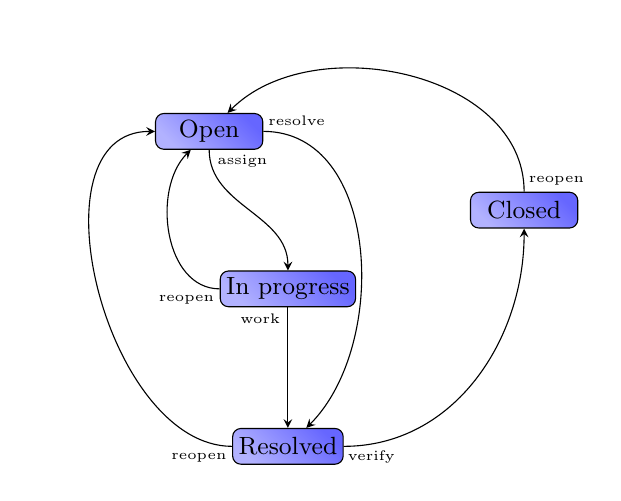
\begin{tikzpicture}
\tikzstyle{status}=[draw,rectangle,shading=axis,left color=blue!30!white, right color=blue!60!white,shading angle=135,anchor=north,rounded corners=3,fill=yellow,inner sep=.5ex,minimum width=9ex,minimum height=3ex]
\tikzstyle{every path}=[draw,->,>=stealth]

\node[status] (open) at (0.0,4.0) {\small{Open}};
\node[status] (wip) at (1.0,2.0) {\small{In progress}};
\node[status] (resolved) at (1.0,0.0) {\small{Resolved}};
\node[status] (closed) at (4.0,3.0) {\small{Closed}};

\onslide<2->{\path (open) to[out=-90,in=90] (wip);}
\onslide<3->{\path (wip) to[out=270,in=90] (resolved);}
\onslide<4->{\path (resolved) to[out=0,in=270] (closed);}
\onslide<5->{\path (resolved) to[out=180,in=180] (open);}
\onslide<6->{\path (wip) to[out=180,in=225] (open);}
\onslide<7->{\path (open) to[out=0,in=45] (resolved);}
\onslide<8->{\path (closed) to[out=90,in=45] (open);}

\onslide<2->{\node[xshift=12,yshift=-4] (label_assign) at (open.270) {\tiny{assign}};}
\onslide<3->{\node[xshift=-10,yshift=-4] (label_work) at (wip.270) {\tiny{work}};}
\onslide<4->{\node[xshift=10,yshift=-4] (label_verify) at (resolved.0) {\tiny{verify}};}
\onslide<5->{\node[xshift=-12,yshift=-4] (label_reopen_resolved) at (resolved.180) {\tiny{reopen}};}
\onslide<6->{\node[xshift=-12,yshift=-4] (label_reopen_wip) at (wip.180) {\tiny{reopen}};}
\onslide<7->{\node[xshift=12,yshift=4] (label_resolve) at (open.0) {\tiny{resolve}};}
\onslide<8->{\node[xshift=5,yshift=4] (label_reopen_closed) at (closed.45) {\tiny{reopen}};}
\end{tikzpicture}
